\documentclass{sigchi}

% Use this command to override the default ACM copyright statement
% (e.g. for preprints).  Consult the conference website for the
% camera-ready copyright statement.


%% EXAMPLE BEGIN -- HOW TO OVERRIDE THE DEFAULT COPYRIGHT STRIP -- (July 22, 2013 - Paul Baumann)
% \toappear{Permission to make digital or hard copies of all or part of this work for personal or classroom use is      granted without fee provided that copies are not made or distributed for profit or commercial advantage and that copies bear this notice and the full citation on the first page. Copyrights for components of this work owned by others than ACM must be honored. Abstracting with credit is permitted. To copy otherwise, or republish, to post on servers or to redistribute to lists, requires prior specific permission and/or a fee. Request permissions from permissions@acm.org. \\
% {\emph{CHI'14}}, April 26--May 1, 2014, Toronto, Canada. \\
% Copyright \copyright~2014 ACM ISBN/14/04...\$15.00. \\
% DOI string from ACM form confirmation}
%% EXAMPLE END -- HOW TO OVERRIDE THE DEFAULT COPYRIGHT STRIP -- (July 22, 2013 - Paul Baumann)


% Arabic page numbers for submission.  Remove this line to eliminate
% page numbers for the camera ready copy 

\pagenumbering{arabic}

% Load basic packages
\usepackage{balance}  % to better equalize the last page
\usepackage{graphics} % for EPS, load graphicx instead 
%\usepackage[T1]{fontenc}
\usepackage{txfonts}
\usepackage{times}    % comment if you want LaTeX's default font
\usepackage[pdftex]{hyperref}
% \usepackage{url}      % llt: nicely formatted URLs
\usepackage{color}
\usepackage{textcomp}
\usepackage{booktabs}
\usepackage{ccicons}
\usepackage{todonotes}
\newcommand{\mytodo}[1]{\todo[inline]{#1}}
\newcommand{\ie}{\emph{i.e.}}
\newcommand{\eg}{\emph{e.g.}}
\newcommand{\migtool}{MIGtool}
\usepackage{soul}
\usepackage{paralist}
\usepackage{listings}

\usepackage{caption}
\usepackage{subcaption}
\usepackage[super]{nth}
\usepackage{amsmath}

% llt: Define a global style for URLs, rather that the default one
\makeatletter
\def\url@leostyle{%
  \@ifundefined{selectfont}{\def\UrlFont{\sf}}{\def\UrlFont{\small\bf\ttfamily}}}
\makeatother
\urlstyle{leo}

% To make various LaTeX processors do the right thing with page size.
\def\pprw{8.5in}
\def\pprh{11in}
\special{papersize=\pprw,\pprh}
\setlength{\paperwidth}{\pprw}
\setlength{\paperheight}{\pprh}
\setlength{\pdfpagewidth}{\pprw}
\setlength{\pdfpageheight}{\pprh}

% Make sure hyperref comes last of your loaded packages, to give it a
% fighting chance of not being over-written, since its job is to
% redefine many LaTeX commands.
\definecolor{linkColor}{RGB}{6,125,233}
\hypersetup{%
  pdftitle={SIGCHI Conference Proceedings Format},
  pdfauthor={LaTeX},
  pdfkeywords={SIGCHI, proceedings, archival format},
  bookmarksnumbered,
  pdfstartview={FitH},
  colorlinks,
  citecolor=black,
  filecolor=black,
  linkcolor=black,
  urlcolor=linkColor,
  breaklinks=true,
}

% create a shortcut to typeset table headings
% \newcommand\tabhead[1]{\small\textbf{#1}}

% End of preamble. Here it comes the document.
\begin{document}

\title{Measuring Interaction Design \\before Building the System: a
  Model-Based Approach}

\numberofauthors{2}
\author{%
  \alignauthor{1st Author Name\\
    \affaddr{Affiliation}\\
    \affaddr{City, Country}\\
    \email{e-mail address}}\\
  \alignauthor{2nd Author Name\\
    \affaddr{Affiliation}\\
    \affaddr{City, Country}\\
    \email{e-mail address}}\\
}

% \author{Giorgio Brajnik\inst{1,2} \and Simon Harper\inst{1}}
% \institute{\textsuperscript{1}Computer Science School\\
% University of Manchester, UK\\
% \email{simon.harper@manchester.ac.uk}\\
% and\\
% \inst{2}Dipartimento di Matematica e Informatica\\
% Universit\`a di Udine, Italy\\
% \email{brajnik@uniud.it}
% }

\maketitle

\begin{abstract}
  Early prototyping of user interfaces is an established good practice
  in interactive system development. However, prototypes cover only
  some usage scenarios, and questions dealing with number of required
  steps, possible interaction paths or impact of possible user errors
  can be answered only for the specific scenarios and only after tedious
  manual inspection.

  We present a tool (MIGTool) that transforms models of the behavior
  of a user interface into a graph, upon which usage scenarios can be
  easily specified, and used by MIGTool to compute possible
  interaction paths. Metrics based on possible paths, with or without
  user navigation errors, can then be computed.  For example, when
  analyzing four mail applications, we show that Gmail compared to
  others has 3 times more shortest routes, has 2x more routes that
  include a single user error, has routes with 13\% fewer steps, but
  has also optimal routes with the smallest probability to be chosen.

  Without MIGTool, this kind of analysis could only be done after
  building some prototype of the system, and then only for specific
  scenarios by manually tracing user actions and relative changes to
  the screens. With MIGTool the exploration of suitability of a design
  with respect to different scenarios, or comparison of different
  design alternatives, can be done after providing only a partial
  specification of the user interface behavior.

  This is made possible by the ability to associate scenarios steps to
  required user actions as defined in the model, by an efficient
  strategy to identify complete execution traces that users can
  follow, and by computing a range of diverse metrics on these
  results. The agile modeling approach that was followed implies that
  relatively little work is needed upfront.

  CONTRIBUTION (asked when submitting the abstract)

  There are three contributions.

  First, we provide means to concisely ground usage scenarios on the
  basis of actions specified in models. This mechanism is general
  enough that can be used also to link tasks or use cases to actual
  behavior of a user interface.

  Second, MIGTool transforms models and scenarios into a graph of
  possible execution paths. Thanks to the special-purpose language
  that is provided to specify scenarios, MIGTool is quite efficient,
  with a time complexiy that is linear with the number of steps in a
  scenario and the number of edges in the graph. We describe the
  language and the algorithm.

  Third, we provide definition of a handful of metrics that are
  objective, precise and that bear upon usability of the resulting
  user interface. They are very general, can be used for most kinds of
  user interfaces that can be modeled with discrete events, and are
  platform independent.

%% EICS submission: #122
%% https://precisionconference.com/~eics16a/updatePaperResponse?userRef=CILXDODXPNF0VESOAFMMC8I16ZO5FR5J&paperNumber=112&emailSent=&error=

  
\end{abstract}

\keywords{Experimental; Evaluation; Statecharts: UML; Metrics; Testing.}

\category{H.5.1}{Information interfaces and presentation (e.g., HCI)}{Multimedia Information Systems}. 
\category{H.5.2}{Information interfaces and presentation (e.g.,
  HCI)}{User Interfaces}. 

\section{Introduction}

% \mytodo{ Subcommittee: Technology, Systems, and Engineering

% People we should pay particular attention to:
% Caroline Appert
% Conversy, St�phane
% Nebeling, Michael

% Keyword we need to pay attention to:
% This subcommittee will focus on technology, systems and engineering
% contributions that enable, improve, or advance interaction. This will
% include software and hardware technologies and systems that enable and
% demonstrate novel interactive capabilities, as well as languages,
% methods and tools for \hl{CONSTRUCTION AND ENGINEERING} of interactive
% systems. Engineering contributions should clearly demonstrate how they
% address interactive systems concerns such as, for example,
% scalability, reliability, interoperability, testing, and
% performance. Systems and technology contributions will be judged by
% their technical innovation and/or ability to connect, SIMPLIFY or
% enrich interactions, for example in intelligent interfaces and
% mobile/ubiquitous computing.
% }
% % 
%\end{quote}


We present an approach that allows a designer to assess interaction
design (IxD) qualities such as efficiency, error-proneness and
recovery from errors. Key importance is given to the ability to
\begin{inparaenum}[(a)]
\item understand how supportive a user interface (UI) is with respect
  to user efficiency;
\item understand how prone the UI is to user navigation
  errors;
\item understand how recoverable the UI is from those errors; and,
\item perform objective quantitative comparison of different designs
  to support construction and engineering of interactive systems.
\end{inparaenum}
All this can be done before developing prototypes of the UI.

To explain our work we present a comparison of four web mail front
ends. We have chosen this domain because it is easy to understand and
yet several questions cannot be easily answered. We applied the same
techniques also in other domains, such as HVAC and other embedded UIs.


Developing good UIs for web or mobile applications is a
complex and expensive endeavor. One reason is the combination of
devices, interaction modalities and workflows that need to be
supported.
%
Adopting Usage Centered Development (UCD) practices is effective, as is
following established design principles~\cite{constantine99}. In
particular, one of the most effective technique is early
prototyping to explore part of the five-dimensional fidelity
prototyping space~\cite{mccurdy06,buxton07}. It is particularly effective when
paired with usability investigations based on user testing or
heuristic evaluations~\cite{preece02,rubin08}.

However, UCD requires prototypes which are usually developed with
certain tasks in mind, and therefore are quite restricted in terms of
depth, breadth, dynamics and data. Furthermore, in addition to the
possible bias introduced by prototypes, usability results are always
surrounded by a cloud of uncertainty, due to subjectivity introduced
by participants and facilitators or by other contingency factors
involved in the analysis. Thus, although a  significant effort
needs to be directed to develop and use prototypes, less than optimal
results are obtained. 

Even worse, several questions cannot be easily
answered. Given one or more potential designs and some usage
scenarios, interesting questions include: ``How many different
routes can be followed by the user to carry out the scenario?'',
``Which are the shortest ones?'', ``If a user makes a mistake, would
he or she be able to recover?'', ``How many steps would the recovery
require?''. When designing and evaluating
embedded UIs (such as when dealing with plane's
cockpits~\cite{conversy07}), other relevant questions include
``How would the above properties change if we add a certain a
widget?'', or ``... if we replace a widget with another?''.  At the
moment, these straightforward questions are quite complicated to
answer. In fact, they require development of prototypes, inspecting
them, manual tracking of which screens and widgets are used at which
stage, and a systematic manual analysis.

This should not be the case, however, because answers to these
questions can be automatically computed. In this way a system can
provide important insights to a designer, and support assessments of
potential user flexibility, user efficiency, error proneness, ability
to recover, compactness and consistency of a design.

Our approach is based on UML statechart models of UIs which are
automatically processed to produce \emph{interaction graphs}. These
graphs are then used to specify interaction scenarios and to unfold
the possible interaction paths (called \emph{execution traces}) that
are compatible with the specific scenarios being considered. Traces
are fed to graph-theoretic computations which produce a
dashboard with different results. Except for development of models and
specification of the desired scenarios, which have to be done
manually, the other steps are totally automatic; models of a design
(such as the ones shown below) can be developed in a matter of a
couple of hours.

Our contribution consists of
\begin{inparaenum}[(a)]
\item the idea of using a UML state machine model to specify
  interaction scenarios,
\item the development of a tool (\migtool, Measuring Interaction
  Graphs Tool) that transforms models and scenario specifications into
  interaction paths, and
\item the definition of metrics that provide concise, precise and
  objective measures of a design.
\end{inparaenum}
The examples presented below show that among four web mail
applications, and with respect to a typical usage scenario, Gmail is
the most efficient and flexible UI, with the best ability to recover
from user errors, but only for users that possess a certain level of
proficiency. In fact, Gmail has the largest number of shortest paths
(when users are supposed to make 0 or 1 error); when users make 2 or
more errors the number of paths drops significantly, reducing the
error-proneness of the UI; on the best case, Gmail features also the
shortest paths, requiring 13\% fewer steps; however, the probability
that a user hits an optimal path with Gmail is 10 times smaller than
the best of the other applications, and the probability that a random
walker hits a state that is not due to an error is 10\% smaller than
the best of the other applications.
%
These values suggest that Gmail offers more ways to accomplish tasks
included in the scenario, that comparably more of these ways do not
involve extra steps, that they require fewer steps, and that it might
be more difficult for novice users to exploit the most efficient
ways. Further inspections show that some differences are due to the
slightly different interaction structures adopted for uploading
messages. If Gmail didn't exist yet, by using \migtool\ its designers
could obtain these answers well before developing prototypes and
performing usability studies.

Other examples shown below show what is gained when a new feature is
added to an embedded system.

\section{Background}
\label{sec:background}

The literature on using state-transition networks for specifying or
analyzing the behavior of UIs is vast. We conducted a systematic-style
literature review, using Google Scholar and queries with combinations
of these phrases: ``user interface'', ``path analysis'', ``user
trace'', ``interaction trace'', ``navigation'', ``markov chain'',
``markov model'', ``state transition'', ``statechart'', ``metric'',
``measure''. For each query we analyzed title and abstract of the
first 50 hits and appraised their relevance based on whether the paper
discusses approaches for measuring user interfaces in the context of
usability and on the basis of a state transition model. This resulted
in 78 full-text papers that were later on re-analyzed against the same
criterion, leading to several of papers mentioned below.
%
Many papers deal with testing user interfaces, and problems related to
generating execution traces as a means to assess coverage of a test
suite~\cite{ammann2008introduction,briand2005:test:uml}. They were
excluded from the review.

Usage of state-transition networks to model UI behavior in order to
draw usability conclusions dates back at least to~\cite{parnas69}. In
it, Parnas claimed that several kinds of usability problems would not
occur if the designer adopted a design framework where states and
their transitions are made explicit.

In many cases \emph{statecharts} are used, a generalization of finite
state automata.  Horrocks showed how statecharts can be used to model
and specify the dynamics of typical desktop
UIs~\cite{horrocks99}. While providing many interesting insights on
how and why one should use statecharts to do so, this nice work does
not address how such a specification could be \emph{automatically}
processed.
%
This idea was later on expanded by Thimbleby~\cite{thimbleby07};
statecharts are seen as crucial representations that allow a designer to
fully appreciate how devices behave. The overall claim is that ``If
you don't understand the logic conveyed by a statechart model of a
user interface, then you don't understand the behavior of the user
interface''.

WebML~\cite{ceri:00} is one of the most successful model-driven
approaches to web development (UIs and backend systems), with
industrial traction and a large number of publications. The language
is based on state transitions and is targeted to automatic generation
of data-intensive web applications.  %WebML encompasses different
%meta-models, independent from the technologies used to deliver the
%final application. % The WebML
% meta-model provides relatively few primitive units that can be
% combined to generate quite complex interactions; the modeling language
% is thus powerful and concise.  
Many other similar approaches involve or are based on task or activity
models~\cite{mori02,silva03:umli,koch02:uwe,gomez01,melia08}.
%
A recent OMG standard, called Interaction Flow Modeling Language
(IFML)~\cite{ifml13}, derives from WebML and focuses specifically on
user interaction. IFML is a language for specifying the structure of a
user interface and its behavior. It offers most of the abstractions
that are available in statecharts, mixed with the ability to specify
so-called ``components'' that are used to display and manipulate data
(to display details of a item, to display or select lists of items, to
input an item). None of these approaches focus directly on measures of
usability.

A rather different route for the problem of generating UIs is followed
in~\cite{heymann2007formal}. Authors assume that the UI to be generated
is used to supervise and to monitor an underlying machine (\eg,
autopilot of a plane) which is modeled as a statechart. After assuming
that the behavior of the UI can also be modeled as a statechart, they
devised an algorithm that checks whether the two models are
compatible, and that refines the UI model so that its states and
transitions are minimized while still allowing a correct manipulation
of the underlying machine. Application of such a technique leads to
UIs that are correct by-construction.

In~\cite{conversy07} the Interactive Cooperative Objects formalism is
discussed, which is based on Petri nets, yet another state transition
formalism.  It is used to enrich the ARINC 661 specification of
Cockpit Display System so that the semantics of widgets can be
expressed and the behavior of a UI be formally analyzed.

%  that are now under provides precise information
% for communication protocol between application (called User
% Applications) and user interface components (called widgets) as well
% as precise information about the widgets themselves. However, in ARINC
% 661, no information is given about the behaviour of these widgets and
% about the behaviour of an application made up of a set of such
% widgets.  The Interactive Cooperative Objects (ICOs) formalism is a
% formal description technique dedicated to the specification of
% interactive systems [4, 11]. It uses concepts borrowed from the
% object-oriented approach to describe the structural or static aspects
% of systems, and uses high-level Petri nets [8] to describe their
% dynamic or behavioural aspects.

Finite state representations have been used also as a conceptual
framework for writing the code of widgets so that events and event
handlers in the UI can more easily be conceived, developed and
verified (\eg, \cite{appert2008swingstates}). 


% in java, FSA used as a conceptual framework to write the code of
% widgets so that events and event handlers in the ui can more easily be
% conceived, developed and verified.

% They say: StateCharts were used in the StateMaster User Interface
% Management System [40], and a variant of them specifically tailored to
% designing user interfaces was used in the more recent HsmTk toolkit
% [18]. StateCharts however are significantly more complicated and hard
% to learn than plain state machines, and our experience is that user
% interface designers and developers have difficulties exploiting their
% power. Other approaches include Petri Nets [41], which have also been
% used to specify user interfaces, for example in the PetShop system
% [42]. Here too, the learning curve is steep, making the adoption of
% such a model by developers difficult.

% With SwingStates, any number of state machines can run simulateneously. A state machine
% can be active, i.e., handling the events it receives, or inactive,
% i.e., ignoring events

% We adopt a similar apporach, but using UML state machine (which are
% more powerful than FSA) for conceiving, guiding development, analysis
% and verification of the behavior of the entire app.

% Nebeling says:\cite{nebeling2011metrics}

% Despite the fact that screen sizes and average screen resolutions have
% dramatically increased over the past few years, little attention has
% been paid to the design of web sites for large, high-resolution
% displays that are now becoming increasingly used both in enterprise
% and consumer spaces. We present a study of how the visual area of the
% browser window is currently utilised by news web sites at different
% widescreen resolutions. The analysis includes measurements of space
% taken up by the article content, embedded ads and the remaining
% components as they appear in the viewport of the web browser. The
% results show that the spatial distribution of page elements does not
% scale well with larger viewing sizes, which leads to an increasing
% amount of unused screen real estate and unnecessary scrolling. We
% derive a number of device-sensitive metrics to measure the quality of
% web page layout in different viewing contexts, which can guide the
% design of flexible layout templates that scale effectively on large
% screens.

% The purpose of ARINC 661 specification (ARINC 661, 2002) is to define
% interfaces to a Cockpit Display System (CDS) used in interactive
% cockpits that are now under

% application of a formal description technique to the various elements
% of ARINC 661 specification within an industrial project. This formal
% description technique called Interactive Cooperative Objects defines
% in a precise and non-ambiguous way all the elements of ARINC 661
% specification. The application of the formal description techniques is
% shown on an interactive application called MPIA (Multi Purpose
% Interactive Application). Within this application, we present how ICO
% are used for describing interactive widgets, User Applications and
% User Interface servers (in charge of interaction techniques). The
% emphasis is put on the model-based management of the feel of the
% applications allowing rapid prototyping of the external presentation
% and the interaction techniques.

% The Interactive Cooperative Objects (ICOs) formalism is a formal
% description technique dedicated to the specification of interactive
% systems [4, 11]. It uses concepts borrowed from the object-oriented
% approach to describe the structural or static aspects of systems, and
% uses high-level Petri nets [8] to describe their dynamic or
% behavioural aspects.

% The Interactive Cooperative Objects (ICOs) formalism is a formal
% description technique dedicated to the specification of interactive
% systems [4, 11]. It uses concepts borrowed from the object-oriented
% approach to describe the structural or static aspects of systems, and
% uses high-level Petri nets [8] to describe their dynamic or
% behavioural aspects.

A review of usability measuring practices~\cite{hornbaek2006current}
lists, under the headings \emph{measures of efficiency/usage
  patterns}, number of keystrokes, mouse clicks, and visited objects
as possible metrics. The notion of \emph{deviation from optimal
  solution} is discussed only in the context of tools for route
planning in 3D navigation. In this paper we provide our own definition
of deviation, which applies to interaction with the UI; we provide
also our notion of execution traces across states of the UI, and the
length of these traces can be used as a measure of efficiency.

Lostness~\cite{smith1996lostness,otter2000lostness} is one of the few
metrics for measuring the degree to which users become lost in the
information space, and therefore considers the notion of
\emph{deviation}. Defined specifically for hypertext systems, lostness
is a user performance measure which is a function of the number of
visited nodes, the number of different nodes that were visited nodes,
and the number of required nodes. This measure of efficiency is
usually applied to traces of actual users, and is argued to be
suitable for hypertext systems because the predominant task is
browsing information, rather than trying to achieve specific goals. It
is suitable therefore when some of the following three assumptions can
be relaxed: that there is a task to complete, that there is a correct
way to carry it out, that the purpose of the system is to support
users to carry out their tasks. 

A usability analysis method capable to analytically predict task
completion times from a storyboard of the UI is
CogTool~\cite{bellamy2011cogtool}. CogTool relies on the ACT-R
cognitive modeling engine, and allows a designer to setup a
low-fidelity prototype of the UI. After deciding which interaction
modality and which widgets are used to implement actions, the designer
gets an estimation of how long an experienced user would
spend on each step. CogTool takes care of adding extra ``mental''
steps, such as ``think'' steps, before certain patterns of provided
steps, according to the cognitive theory underlying ACT-R. As a
result, users of CogTool obtain the breakdown of the times required by
each of the steps. Our method is weaker in terms of cognitive validity
and in terms of precision of the output: it does not provide expected
completion times. However, with our method one can analyze a large
part of the UI, get information about possible problems in some areas,
and only then devolve more resources in building storyboards and
in making assumptions regarding widgets so that specific execution
paths previously identified can be analyzed with CogTool. In a sense,
the output of our method could be used to make informed decisions as
to what to analyze with CogTool.

Markov models, \ie\ directed graphs where edges leaving a vertex are
associated to a probability distribution, were used
in~\cite{thimbleby2001markov}, as a means to perform usability
analysis as early as possible, even before building prototypes of the
UI. Vertices represent states of the UI and edges correspond to user
actions (such as pressing a push-down button).  Probabilities can be
used as a model of user knowledge: equiprobable actions correspond to
a knowledge-free user, whereas when some actions have a very low
probability it means that for that user the action is unlikely to be
executed. Simple mathematical operations on the transition matrix of
the model give the probability that after $n$ steps from a given
initial state the UI is in a given state. With Markov models, by
manipulating probabilities, the designer can plot the number of
required steps as a function of how close the probabilities are to the
designer's ``perfect'' knowledge.  Examples discussed in the paper
cover several devices, ranging from a simple torch (with 4 states), a
microwave cooker (6 states), a mobile phone (152 states); those are
all push-down devices with a fixed set of buttons. This is obviously
not the case for UIs of information systems, where buttons may change
screen by screen. This makes it more difficult to specify the
transition matrix. 
%
Our approach is based on statecharts, a language that in practice is
more powerful than Markov models, making it easier to specify the UI
behavior, especially in cases where the set of buttons change over
time. While our examples do not make use of probabilities, this is
very easy to cope with (see the Discussion at the end of the paper for
some of the benefits that doing this could bring). Similarly
to~\cite{thimbleby2001markov}, our approach could be used when
conservative results that do not rely on psychological assumptions are
sought.


A discussion of social network analysis metrics applied to interaction
design is provided in~\cite{thimbleby09:sna:eics09}. Once more, a UI
is modeled in terms of directed graphs (vertices are states and edges
are actions), and various centrality metrics are used to draw
conclusions that bear upon usability. For example, centrality measures
(such as Sabidussi, eccentricity, betweenness) can be used to identify
states that are good places to start from to get to other
states. Other metrics, such as edge betweenness, can be used to
identify actions that are important because most of the shortest paths
go through these actions. The paper presents compelling examples of
using this technique to identify shortcomings in the design of
infusion pumps.
%
In our work we automatically generate graphs from statechart models,
and on some of them computed these metrics. We were not able to draw
sensible conclusions from the values we obtained (for example from the
models presented below). One possible explanation rests on the
different types of models: in our case they reflect the variety and
flexibility with which ``buttons'' can be used in modern web
applications. For infusion pumps the UI is more constrained in how a
task can be carried on, and this difference might reflect on the
usefulness of those metrics.

In~\cite{hilbert2000} several approaches to analyze streams of user
events are discussed and compared. It is interesting to realize that
this is, in a sense, the inverse problem of the one we tackle in this
paper: we want to compute a subset of the possible streams of user
events given a specification of the UI, rather than trying to abstract
general properties from streams of events.


% Voida\cite{voida} says:
% We describe an alternative model for organizing the
% desktop interface-activity-based computing-and
% identify a series of high-level system requirements for
% interfaces that use activity as their primary organizing
% principle.

% We could mention this work when we introduce scenarios, and say that
% people inventing these new metaphors could take advantage of our
% metrics if they model 2+ apps. 

% Eg. they say: Requirement 2. Activity-based systems should provide
% lightweight mechanisms to create, change, and alter
% activities, since heavyweight interaction techniques are
% likely to deter adoption and use.

% eg Requirement 7. Because information sharing is a
% �common case� in knowledge work, lightweight sharing
% capabilities should be integrated directly as a first-class
% interaction technique. 

\section{Generation of interaction traces}
\label{sec:traces}

In this section we provide a description of how \migtool\ computes
execution traces.  They are paths (\ie, sequences of connected states
of the model) that users can follow when performing a given scenario.
The generation process encompasses the following steps:
\begin{inparaenum}[(1)]
\item automatic flattening of the statechart model;
\item manual definition of the interaction scenario;
\item automatic generation of execution traces; and
\item interactive analysis of results.
\end{inparaenum}

\subsection{Processing models }

\migtool\ takes as input UML statecharts, which are a generalization
of finite state automata (FSA), with an expressive language that
includes hierarchic levels of abstraction, concurrent regions, states
and pseudostates, guards, and an extended state notion based on an
arbitrary underlying computational model.  Harel, the inventor of
statecharts, gives an interesting retrospective view of how they were
invented, back in early eighties, and why they were appealing also to
non experts~\cite{harel09}.  For the sake of brevity, we refrain from
describing them here in detail; the interested reader is referred to
the UML standard~\cite{uml25} or some of the textbooks that deal with
them, like~\cite{samek09}.

By using statecharts, the behavior of UIs can be represented by
associating states to screens and particular configurations of
widgets, and transitions to actions performed by users or by the
system itself. In the classification reported in~\cite{hilbert2000},
actions belong to the ``abstract interaction events'' category.

Because statechart models take advantage of abstraction features and a
rich set of connecting pseudostates, they are not suitable to be
directly processed to compute metrics. For this reason, \migtool\
first \emph{flattens} the model. Flattening is a process often used
when statecharts have to be automatically
processed~\cite{briand2005:test:uml}, and it means to produce a FSA
that is behaviorally equivalent to the original statechart, with no
hierarchy between states and no concurrent regions. In most cases this
leads to an exponential number of states and transitions in the FSA,
but because the process is completely automatic and there is no need
to manually inspect the resulting FSA, this aspect is in many cases
not relevant.  \migtool\ produces an XML representation (graphML) of
the resulting FSA, the \emph{interaction graph}. It is a directed
multigraph\footnote{A directed multigraph is a directed graph such
  that there are 2 or more edges that have the same end points. Cycles
  are paths that include 2 or more occurrences of the same
  vertex. Loops are edges that start and end on the same
  vertex. ``Geodesic path'' is a synonymous term with ``shortest
  path''.}, potentially with cycles and loops, with edges that are
labeled with the name of the corresponding action. In the following we
will be using as synonymous the terms state/vertex, and action/edge.

\subsection{Defining usage scenarios}

Because in all but the most trivial interaction graphs there are
cycles, the set of possible interaction traces is infinite. For this
reason, scenarios need to be defined and used as constraints on the
possible execution traces that can be generated.  Users of \migtool\
define interaction scenarios by specifying key steps (called
\emph{bridge sets}) that users are expected to go through; we call
this process \emph{grounding usage scenarios on models}. Each bridge
set is specified by selecting a subset of the edges of the interaction
graph. In general a specification includes an initial state and a
sequence of bridge sets. For example, to specify a scenario for
replying to an email message, one could select all the edges
associated to the action \texttt{reply} (bridge set 1), followed by
edges labeled with \texttt{typeBody} (bridge set 2), followed by edges
labeled with \texttt{send} (bridge set 3). A well formed bridge set
consists of 1 or more edges (an empty bridge set would make the
scenario unviable). In this way scenarios with cycles can be
formulated (\eg, reply twice to two messages). A \emph{stage} of a
scenario comprises two consecutive bridge sets.
%
To cope with multi edges, the interaction graph is \emph{simplified}:
all edges between a   pair of vertices are merged into a single one,
whose label includes the original ones.

\subsection{Searching traces}

Quite expressive languages can be conceived for grounding scenarios
(\eg, regular expressions on sequences of action names). But such
expressivity bonus needs to be balanced with computational
tractability: even models with a dozen states might correspond to interaction
graphs with several hundred states and several thousand edges, leading
to an enormous number of possible traces to filter even for scenarios
with just a few stages.

To cope with this we implemented a trace searching algorithm that
processes each of the stages sequentially, starting from the initial
initial state. Given a bridge set $B_i$, the algorithm does a
breadth-first search of all the geodesic paths that connect
\emph{each} of the ending vertices of edges in $B_i$ with \emph{some}
of the starting vertices of edges in $B_{i+1}$. If some bridge in
$B_{i+1}$ cannot be reached, then it is dropped from further
searches. \migtool\ creates a new graph from the geodesic paths found
for each stage, and then joins these graphs so that geodesic paths
found for stage $i$ are joined with those of ${i+1}$. These global
paths, connecting the initial state to reachable bridges of the
last bridge set of the scenario are called \emph{execution traces}.

Notice that a scenario specifies only the desired occurrences of
actions, not all the necessary ones. For example, if the model
prescribes that in order to \texttt{view(message)} while reading
another one, one has to \texttt{goBack} to the inbox first, a scenario
specifying two consecutive \texttt{view(message)} would lead to traces
that include also the \texttt{goBack} action, even if that step is not
explicitly specified in the scenario. It is the task of \migtool\ to
unfold paths in the graph and search all the geodesic paths that
connect the desired user actions.

\subsection{Detour traces}
The algorithm described so far finds (some of) the global paths
connecting the initial state to one or more bridges for each of the
specified stages. The globally shortest paths are included in the
solution, together with other viable alternatives. These traces are
called \emph{detour order 0} traces.

\migtool\ is used to process a model and a scenario
and to generate execution traces of detour order = 0,
..., H. 
For each stage, up to a maximum detour order $H$, the search algorithm
creates traces with detour order $k+1$ by collecting the set $D_k$ of states
with order $0$ up to $k$, and by identifying the neighbors ($N_k$)
of $D_k$ ($N_k$ is the set of states  not included in $D_k$ that are
connected through an edge to some state in $D_k$). Edges connecting
$D_k$ with $N_k$ represent deviations that users might follow, and
geodesic paths between $N_k$ and $D_k$ constitute recovery paths that
users might follow to complete the scenario from states in
$N_k$. These deviations and recovery paths are joined and constitute
the traces of order $k+1$.  It could happen that
for some state in $N_k$ there is no path leading to any vertex in
$D_k$: in such a case the deviation leads to a dead end that prevents
the user to complete the scenario.

The time complexity of the search algorithm is
$\mathcal{O}(KM(E+V)))$, where there are $K$ bridge sets, their mean
size is $M$, the interaction graph has $V$ vertices and $E$
edges. Therefore it scales well with the size of the
interaction graph and/or complexity of the scenarios. In practice for
interaction graphs consisting of about 10000 edges and a dozen of
bridge sets, on a low-cost PC it takes about 20 seconds to generate
traces of order 0 to 3.


\section{Comparing applications}
\label{sec:casestudy}

In this section we describe some examples of the results that can be
obtained with \migtool, based on well known web mail clients, namely
Gmail, Horde, SquirrelMail and Roundcube. We chose these examples
because they are well known, and therefore are easy to describe and
understand. And yet, despite email being a very well understood
domain, the kind of questions that can be posed and the answers that
are found provide interesting insights on some of the usability properties of
these applications.

\subsection{Models and scenarios}
\label{sec:models-scenarios}

Models of the four applications have been manually defined. In order
to support a fair comparison, all four models cover the same set of
use cases: listing the content of the inbox, reading a message or
conversation, replying to a message, composing and sending a new
message.

Figure~\ref{fig:model} shows part of the model of Gmail. At some
point, a user is viewing all the conversations of the inbox (state
\texttt{viewingConversations}); available actions include moving to
the next or previous block of conversations, refreshing the list, or
opening a specific conversation (transition
\texttt{open(conversation)}). This transition (which is assumed to
occur when the user clicks on one of the visible conversations) leads
to the state \texttt{viewingAConversation}, where the behavior of the
system is defined by a more detailed state machine. By default the
user is viewing a conversation, but by performing the \texttt{reply}
action the UI moves to a state called \texttt{replying}, where the
body of the reply can be typed, the subject can be changed, or another
addressee can be added.

Notice that this behavior ``happens'' in one of the two concurrent
regions specified by this model. In parallel to this, the user can
either be reading messages (state \texttt{reading}) or may be
composing a new message (state \texttt{composing}). In the latter case
the user can independently add recipients, attachments, write the body
or subject of the message; and send or cancel it.

\begin{figure*}[tbh]
  \centering
  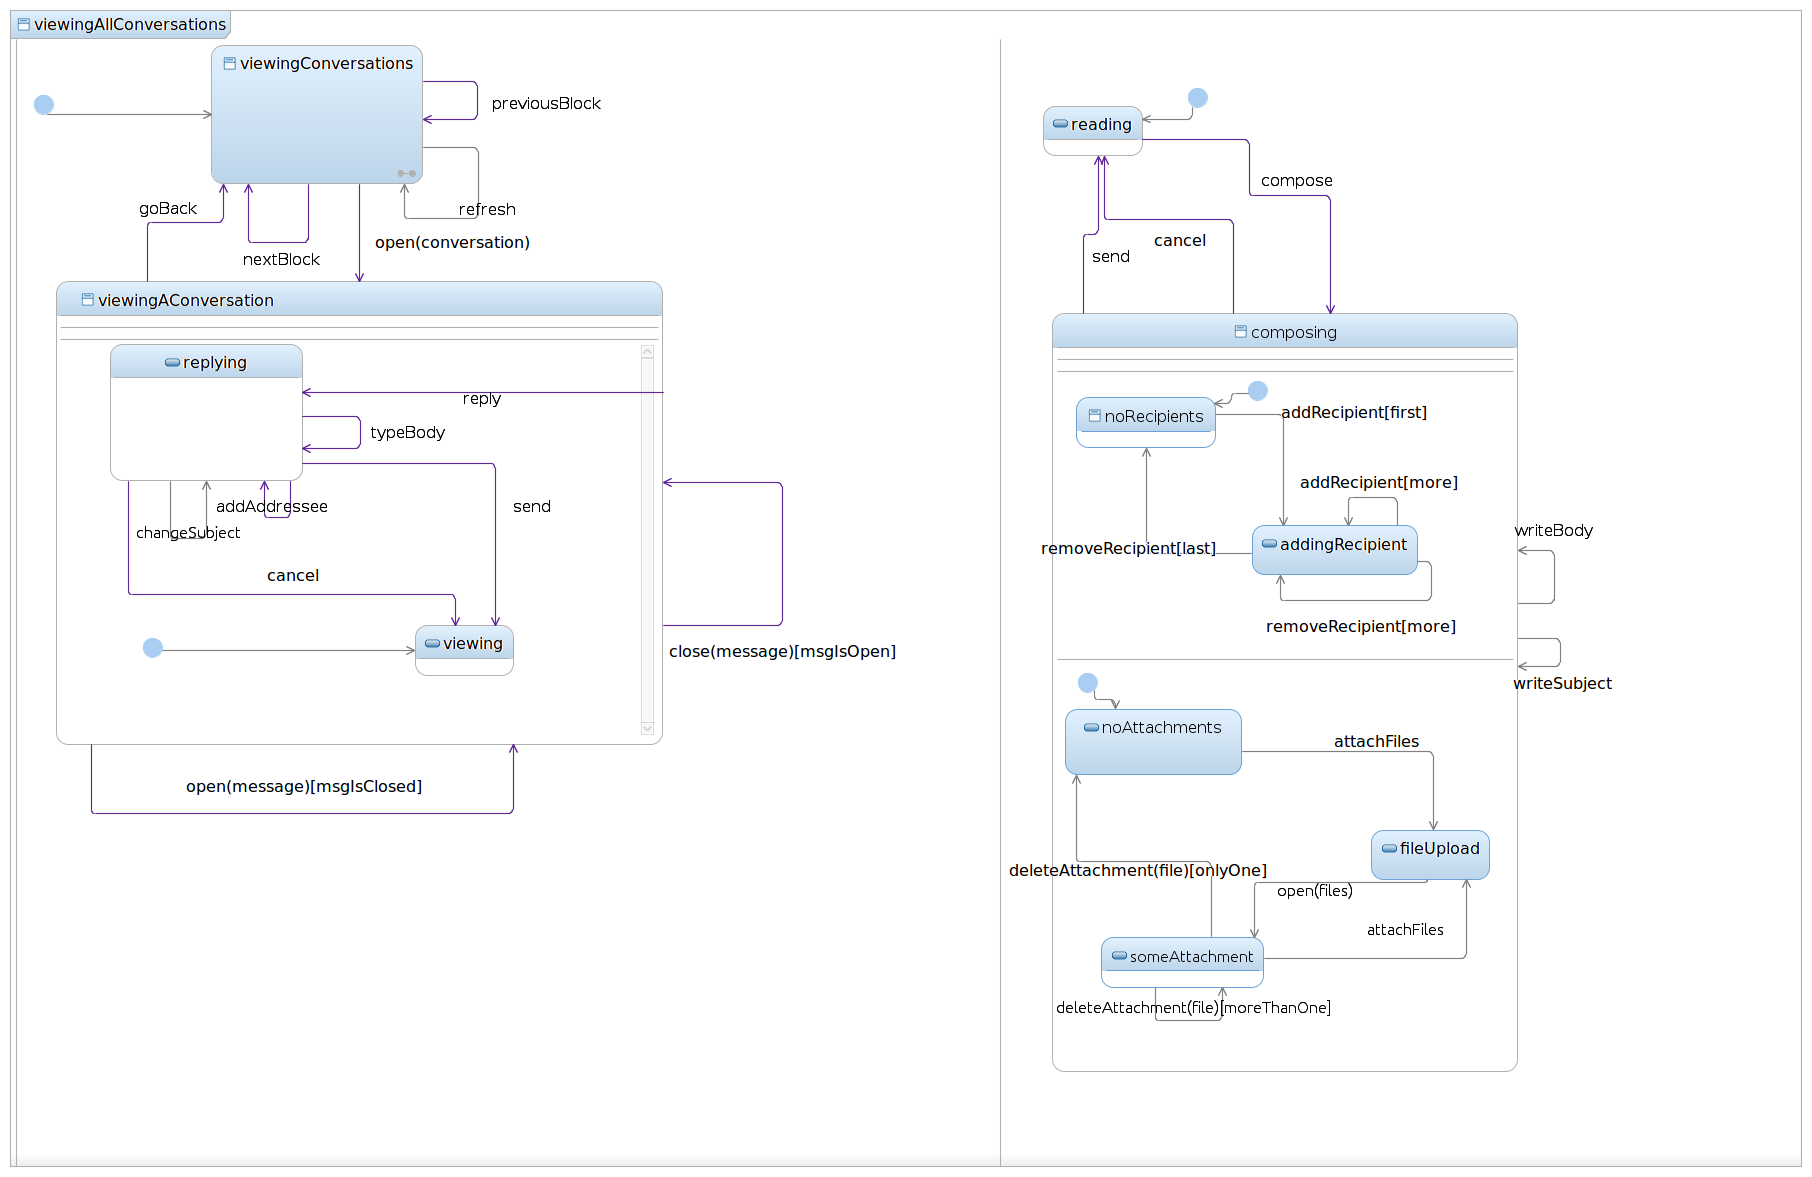
\includegraphics[width=1.05\linewidth]{figures/gmail_2.png}
  \caption{Part of the Gmail model.}\label{fig:model}
\end{figure*}

The model that we show here is part of what we used in the examples
reported below. The actual model that we used consists of 
24 states, 12 pseudo states, 12 regions, and 61 transitions. 

The flattening process, which takes a couple seconds on a low-cost PC,
produces a directed multigraph with 47 vertices and 634 edges; when
simplified by collapsing multiple edges, the number of edges drops to
312. Each vertex represents one of the possible combinations of simple
states in any of the regions that can be active at the same time.

Similar models and corresponding graphs were produced for the other
three applications. 



\subsection{Analysis of interaction designs}
\label{sec:analysis}

Inspection of the interaction graph is not particularly useful because
even for small graphs like the one obtained from our Gmail model no
particular structure is evident that was not known from the
model. Figure~\ref{fig:gom} shows a plot using a circular layout of
the 47 states: because of the large number of cycles that exist among
states, edges form an intricate web of possible action sequences. We
believe this in practice greatly reduces usefulness of typical network
analysis metrics, such as \emph{betweenness, eccentricity, page-rank,
  eigenvalue} centrality measures.

\begin{figure}
  \centering
  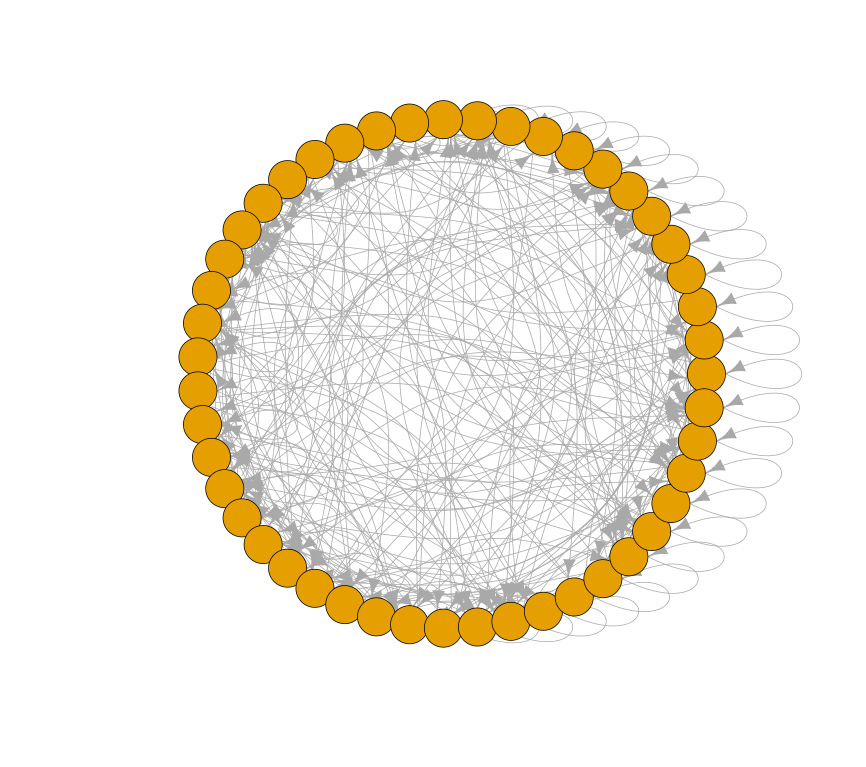
\includegraphics[width=\linewidth]{figures/gom.png}
  \caption{Interaction graph obtained from the Gmail model.}
  \label{fig:gom}
\end{figure}


To be able to obtain results that bear upon usability, we process
further the graph, by specifying scenarios and computing traces.  The
following fragment of R code specifies the bridge sets of the chosen
scenario: it comprises, in the given order, two occurrences of
\texttt{open(conversation)}, followed by \texttt{reply}, followed by
\texttt{typeBody}, etc.: \lstset{language=R}
\begin{lstlisting}
edgesWithLabel(gmail,"open(conversation)"),
edgesWithLabel(gmail,"open(conversation)"), 
edgesWithLabel(gmail,"reply"),
edgesWithLabel(gmail,"typeBody"),
edgesWithLabel(gmail,"send"),
edgesWithLabel(gmail,"compose"),
edgesWithLabel(gmail,"addRecipient"),
edgesWithLabel(gmail,"open(files)"),
edgesWithLabel(gmail,"writeBody"),
edgesWithLabel(gmail,"writeSubject"),
edgesWithLabel(gmail,"send")
\end{lstlisting}
In plain language such a scenario means opening a conversation,
opening a second one, replying to the last message of the
second conversation by typing the body of the response, sending it, and then
composing a new message by adding a recipient, an attachment, typing
the body and subject, and finally sending it.

The execution traces for such a Gmail scenario, with a detour limit of
3, consist of a graph with 474 vertices and 1753 edges. These traces
entail 12 possible geodesic paths with order 0, 82 with order 1, 30
with order 2 and 33 with order 3. Figure~\ref{fig:numpaths} shows the
number of paths obtained for the four applications, split by detour
order.


\begin{figure}[tbh]
  \centering
  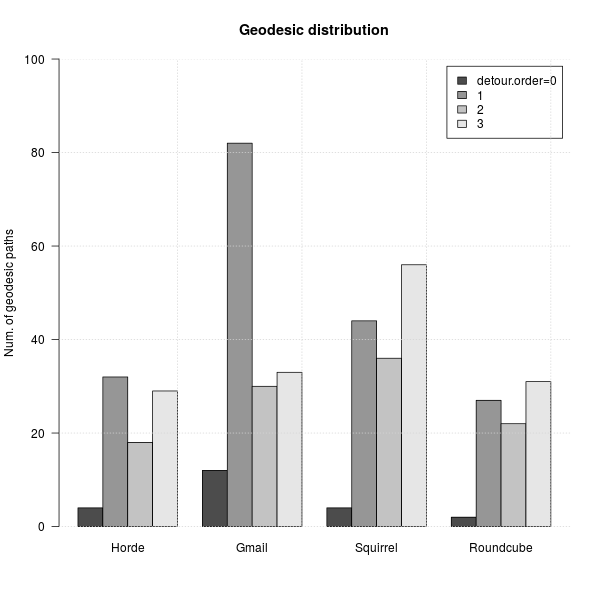
\includegraphics[width=\linewidth]{figures/gpd.png}
  \caption{Number of geodesic paths split by detour order.}
  \label{fig:numpaths}
\end{figure}

% tot.hom
% ##     N min max        M       rel  N
% ## d0  4  15  18 15.75000 0.2539683  4
% ## d1 32  16  22 17.94531 1.7831955 36
% ## d2 18  18  24 19.25000 0.9350649 54
% ## d3 29  19  24 19.95690 1.4531317 83
%  tot.gom
% ##     N min max        M       rel   N
% ## d0 12  13  17 15.08333 0.7955801  12
% ## d1 82  14  24 19.11179 4.2905456  94
% ## d2 30  16  25 20.57778 1.4578834 124
% ## d3 33  17  26 21.51515 1.5338028 157
%  tot.sqm
% ##     N min max        M       rel   N
% ## d0  4  15  19 17.00000 0.2352941   4
% ## d1 44  16  24 19.77273 2.2252874  48
% ## d2 36  18  26 20.88889 1.7234043  84
% ## d3 56  19  25 21.64286 2.5874587 140
%  tot.rcm
% ##     N min max        M       rel  N
% ## d0  2  15  18 16.50000 0.1212121  2
% ## d1 27  16  24 19.07407 1.4155340 29
% ## d2 22  18  25 20.18182 1.0900901 51
% ## d3 31  19  24 21.04839 1.4727969 82

Gmail has the highest number of order 0 and 1 traces; it has the
highest difference between the number of order 0 and 1, and between
order 1 and 2 (at least 3 times as many order 0 paths than any of the
other applications, and at least twice as many order 1 paths as the
any of the other applications).  In other words, Gmail offers 3 times
as many error-free alternative paths to accomplish the scenario, which
indicates that users might more easily follow one of those paths, than
when using other applications.  Notice that Roundcube has the smallest number
of order 0 paths (2 of them), which means that users are not given
much flexibility and freedom in carrying out correctly the scenario.
However, Gmail provides also almost twice as many order 1 paths, which
means that users could be more easily induced into an erroneous path
than when using another system (or given more flexibility).
Because the number of order 2 or 3 paths decreases, Gmail reduces
therefore the ``error proneness'' of this UI, for executions that
involve 2 or 3 errors. 

For none of the systems a detour leads to dead-ends.

Figure~\ref{fig:bestcase} shows the length of paths in the best case,
i.e., when users would always choose the shortest route. Gmail offers
the shortest paths across the four detour orders (for order 0 the
length is 13 steps, saving more than 13\% steps compared to other
applications; for order 3 the length is 17 steps; the other
applications are remarkably similar among them).  A plausible
interpretation is therefore that Gmail not only offers many more
error-free paths, but also gives the shortest ones. Users are given
more flexibility and more efficiency.  Because also paths with order 1
or more are the shortest ones among the four applications, Gmail also
makes users more efficient in recovering from errors.  

\begin{figure}[htb]
  \centering
  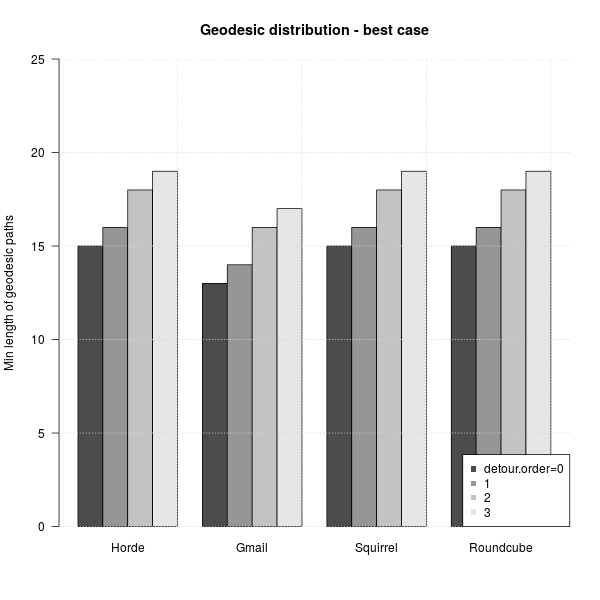
\includegraphics[width=\linewidth]{figures/min-paths.png}
  \caption{Minimum length of  geodesic paths split by detour order.}
  \label{fig:bestcase}
\end{figure}

%Figure~\ref{fig:averagecase} 


% \begin{figure}[htb]
%   \centering
%   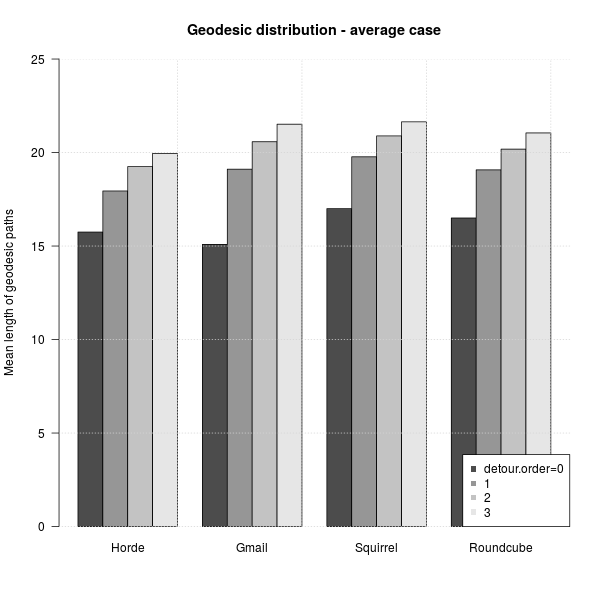
\includegraphics[width=\linewidth]{figures/mean-paths.png}
%   \caption{Average length of  geodesic paths split by detour order.}
%   \label{fig:averagecase}
% \end{figure}

\begin{figure}
  \centering
  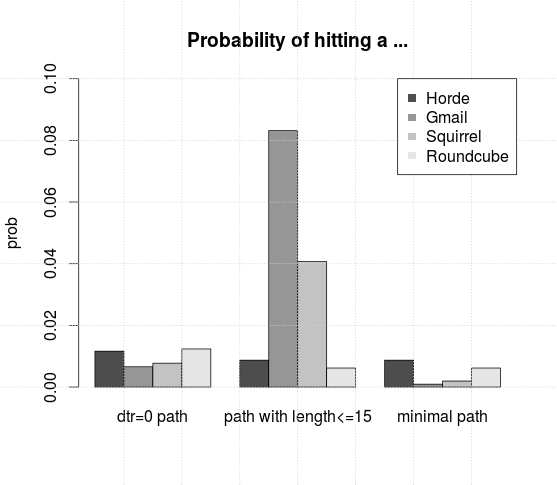
\includegraphics[width=\linewidth]{figures/prob-opt-path.png}
  \caption{Frequency of an optimal path.}
  \label{fig:freqopt}
\end{figure}

To combine these two results, we can easily compute the frequency of
paths having different length. Figure~\ref{fig:freqopt} shows, for
each application, the frequency of order 0 paths, the frequency of
paths with length less or equal to 15 (the minimum length across the
four applications), and the frequency of optimal paths (the shortest
ones). These values show that Gmail users have the lowest probability
to hit an order 0 path (because of the relative large number of order
1 paths made available by Gmail), have the lowest probability of
hitting the shortest paths (10 times smaller than the best of the
other applications), but have the highest probability to hit a
path with length 15 or less.  Thus, the flexibility and efficiency
that can be exploited with Gmail are counterbalanced by the required
knowledge and capability of choosing an optimal path. In particular,
Gmail offers many detours of order 1 which increase flexibility for
some users and might decrease effectiveness for less knowledgeable
ones. 

% >   d=0.050 # 5% chances that a user makes a generic mistake
% >   dprh=detour.page.rank(sc.hom,3,d);dprh
%          0          1          2          3 
% 0.73455373 0.11735984 0.05684419 0.09124223 
% >   dprg=detour.page.rank(sc.gom,3,d);dprg
%          0          1          2          3 
% 0.69210344 0.17697177 0.06228221 0.06864257 
% >   dprs=detour.page.rank(sc.sqm,3,d);dprs
%          0          1          2          3 
% 0.79062415 0.07122957 0.05364190 0.08450438 
% >   dprr=detour.page.rank(sc.rcm,3,d);dprr
%          0          1          2          3 
% 0.76538478 0.08355996 0.06247253 0.08858273 %

Another probabilistic analysis can be performed using page rank, which
computes the probability that a random walk in a graph visits a
certain vertex~\cite{page1999pagerank}. We computed the page rank
(with a damping value of 5\% - meaning that the random walker with
probability 5\% jumps to an arbitrary state and probability 95\%
chooses one of the actions available in the current state) for each
vertex in the graph, and then summed up page rank values for vertices
with different detour order.  Figure~\ref{fig:pr} shows the resulting
sums.


\begin{figure}
  \centering
  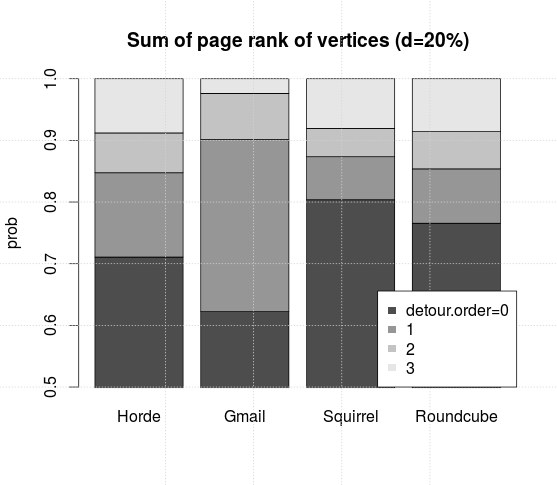
\includegraphics[width=\linewidth]{figures/pr.png}
  \caption{Probability that a random walk visits detour 0, 1, 2 or 3 states.}
  \label{fig:pr}
\end{figure}

With Gmail the probability of visiting an order 0 state is close to
70\%, the lowest among the four applications. But when it comes to
visiting an order 0 or 1 state, the probability increases to 87\%,
which is the highest. Thus, in a comparison of Gmail against
SquirrelMail, a completely random usage of SquirrelMail has 10\% more
probability of hitting an error-free state than Gmail. That advantage
is slightly reduced when considering order 0 and 1 paths, because with
SquirrelMail the probability is 85\% and Gmail it is 87\%.  This means
that somebody with no knowledge on how to use an email front end, when
using Gmail would have 10\% fewer chances of carrying out the scenario
without making any error, as opposed to when using SquirrelMail:
SquirrelMail provides more guidance. Across the four UIs, the
probability of making at most 1 error is approximately the
same\footnote{These results are not very sensitive to the value chosen
  for the damping factor: differences across the four applications are
  stable when $d$ ranges in $[0.05,0.20]$.}.

Manual inspection of the shortest paths indicates that one reason of
the higher potential efficiency offered by Gmail is due to the
fact that users can start composing a new message while reading a
conversation, whereas in other applications an explicit ``close action'' of
the reading activity has to be performed. Another reason relies on the
more streamlined process to attach a file: in Gmail one needs to
select the file(s) and they are automatically uploaded, whereas in
other applications one has to explicitly perform the uploading step
after selecting them.


\begin{figure}
  \centering
  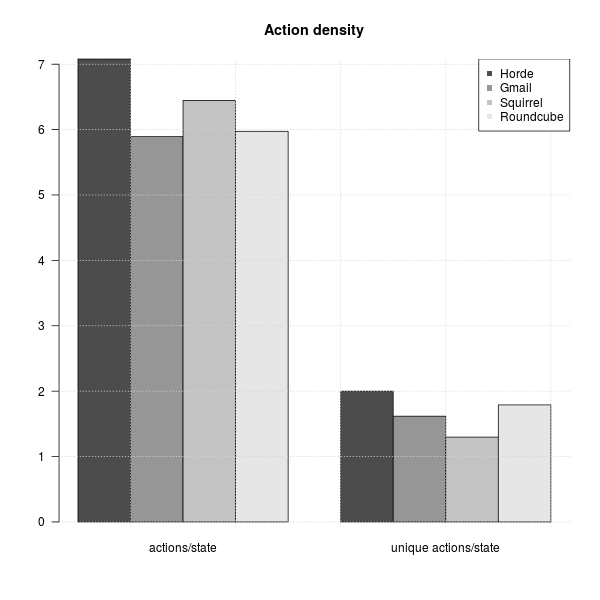
\includegraphics[width=\linewidth]{figures/ad.png}
  \caption{Action density.}
  \label{fig:ad}
\end{figure}

Figure~\ref{fig:ad} shows the \emph{action density} of the four
applications, \ie\ the average number of actions per state involved
in traces, and average number of \emph{unique} actions per state. The
former is an overall measure of the number of options that are made
available by a UI, the latter can be used to analyze how many
\emph{new} options the user is presented with in any state. For our
examples, the values are all in the range between 5.9 actions/state in
the case of Gmail and 7.1 for Horde, and 1.3 unique actions for
SquirrelMail and 2 for Horde. This suggests that Gmail features a more
compact design (fewer actions to do the same things), and SquirrelMail
is even more compact when it comes to the different types of actions;
thus it could be easier to learn.

\subsection{Comparing scenarios}
Previous examples show how \migtool\ can be used to compare different
UIs against the same scenario.  The same kind of analysis can be
carried out to assess how suitable a design is for different
scenarios. For example, a designer might be interested in a comparison
of replying to a message as opposed to composing a new one.

Focusing now on Horde, it turns out that composing a new message
entails many more order 0 paths (154 vs 86), and a comparable number
of higher order paths. The path length in the best case is the same
across the two scenarios, but in the average case composing has a
length of 7.75 steps compared to 8.5 for reply. Probability of hitting
an optimal path is 4 times higher for compose.


This means that users will have twice as much many choices between 
correct paths when composing a new message rather than simply
replying to a read one. On average, when composing, users could be
9\% more efficient, and they are 4 times more likely to do the right
things. Thus, Horde is more suitable for composing new messages than
it is for replying to existing ones.


\subsection{Adding features}

Execution traces can be used also to assess what is the effect of
adding a widget or feature to an existing UI.  For example, we studied
some cruise control features of cars. One of the examples is system
S\footnote{There is no need to disclose the actual brand.}, where the
driver can engage the system, and once it is engaged, speed can be
increased or decreased with small or large steps. Of course the system
can also be disengaged (by pressing the brake pedal, for example).
System A is more elaborate, as it includes also a memory function:
when it is disengaged it remembers the current speed, which can be
recalled later on.  There are two ways to re-engage it: one by setting
a new speed, and one by recalling the previous one. In addition, if
the car drives for more than 5 minutes at a higher speed than the set
one, system A automatically disengages.

Thus, one possible design question is ``What are the effects of adding
these functionalities?'' in a typical driving scenario where a speed
is selected, then the system is disengaged, and later on the same
speed needs to be set.

\begin{table}
  \centering
  \begin{tabular}{|c|r|r|r|r|r|r|r|r|}\hline
    System & $N_0$ & $L_0$ & $N_1$ & $L_1$ & p & AD & UAD \\\hline
    S  & 1 & 7 & 8 & 9.4& 11\% & 1.75 & 1.25 \\
    A  & 2 & 4.5 & 7 & 6.8 & 6\% & 2.20 & 1.20 \\\hline
  \end{tabular}\vspace{1mm}
  \caption{Comparison of the two cruise control designs. $N_i$: number
    of execution traces with detour order $i$; $L_i$: average length of
    traces with detour order $i$; $p$: probability to hit the shortest execution
    trace; AD: actions/state; UAD: unique actions/state.}
  \label{tab:data}
\end{table}

When using a scenario for S where we assume that re-setting the speed
is done manually by the driver with 4 actions on ``up'' and ``down''
to approximately get the same speed), the comparison produces the
values shown in Table~\ref{tab:data}. 
System A has 2 alternative optimal paths, their length is 4.5 (36\%
shorter than in S); both systems have a comparable number of detour 1
traces, but again their length in A is  28\% shorter. The probability
of hitting the optimal trace is however twice as large in S, which
features also a more compact design. 
In both cases detours are caused by the possibility of disengaging the
system at the wrong moment.

Therefore we can conclude that:
\begin{inparaenum}[(1)]
\item system A makes users more efficient (an increase of 56\%) for
  the considered scenario;
\item with A there are two possible ways to achieve the scenario, thus
  more flexibility is given;
\item with A the probability of doing the right thing is almost half
  of system S: it might be more difficult to do the right thing
  because more possibilities are offered;
\item system A features a more compact design, with fewer action types
  to be performed at each moment.
\end{inparaenum}




% \begin{table*}[ht]
% \centering
% \begin{tabular}{rllll}
%   Step &Horde & Gmail & Squirrel & Roundcube\\
%   \hline
%   1 & openMessage(msg) & open(conversation) & openMessage(msg) & openMessage(msg) \\ 
%   2 & exitMessage & goBack & exitMessage &  exitMessage \\ 
%   3 & openMessage(msg) & open(conversation) & openMessage(msg) & openMessage(msg) \\ 
%   4 & reply & reply & reply & reply \\ 
%   5 &  typeBody & typeBody & typeBody                       &  typeBody \\ 
%   6 &  send &  send & send                                  & send \\ 
%   7 &  exitMessage &  & exitMessage                  &  exitMessage \\ 
%   8 & compose &compose & compose                        & compose \\ 
%   9 & addReceiver(receiver) &  addReceiver(receiver)  & addReceiver(receiver)   & addReceiver(receiver) \\ 
%   10 & browseFiles          & attachFiles   & browseFiles  & attachAFile \\ 
%   11 & selectAttachments(file) & open(files)  & selectAttachments(file)          &  selectAttachments(files) \\ 
%   12 & update                &  &add   &  upload \\ 
%   13 &  typeSubject          &  typeSubject          &  typeSubject & typeSubject \\ 
%   14 & typeBody &         typeBody                    & typeBody     & typeBody \\ 
%   15 &  send &           send                    &  send        &  send \\ 
%    \hline
% \end{tabular}
% \end{table*}


\section{Discussion}
\label{sec:discussion}

An important issue underlying \migtool\ is the modeling effort that is
needed upfront. Our experience, based on several case studies and some
industrial examples, is that models do not need to be complete
representations of the behavior of the application under
study. By following an agile modeling approach~\cite{ambler02}, models can
be easily developed by one person in less than one day, using any UML
capable design tool. Even more complex models (in our experience up to
150 states and 350 transitions) can be developed and verified in 2-3
days by one person.
Experience in using statecharts to model behavior of UIs is needed
though. Useful suggestions are given in~\cite{horrocks99,thimbleby07}.

UML state diagrams provide a very expressive language, well suited to
specify behavior of UIs based on discrete events. Evidence of this can
also be found in recent OMG standards, such as
IFML~\cite{ifml13}. Even though there are fundamental limits
(inability to handle undo/redo's - because that goes beyond a finite
state representation; inability to handle customizable toolbars -
because that requires models that change at runtime; inability to
handle perceptive UIs - because they are not well suited to be
described in terms of discrete states), in many practical cases they
can be be isolated and/or ignored.

Expressivity of the modeling language means that different designers
are likely to produce different models for the same UI. As a
consequence, it is possible that metrics computed by \migtool\ do depend on different
modeling choices. It is worth mentioning, though, that because of the
flattening process, several differences are reduced (for example,
those dealing with using a different hierarchy of states, or with
distributing differently concurrent regions across states), and 
sensitivity is correspondingly reduced. At the moment, however, we do
not have hard evidence to back this claim.

Differently from other model-based approaches, such as those based on
IFML, \migtool\ uses \emph{only} a model of the behavior of the
UI. Designers do not need to cope with data modeling, nor with
decisions dealing with presentation. In a sense, \migtool\ uses only the
\emph{controller} part of the Model-View-Controller paradigm that is
adopted when developing UIs. Therefore, the designer using \migtool\ to
perform analysis is free from other concerns that in the end affect
usability, and the conclusions that are derived with \migtool\ can be
combined with other results \emph{after} the analysis is
performed. 

In terms of validity of conclusions obtained through \migtool, we can
say that because they are devoid of user behavior assumptions (such as
preferences, skills, interpretations, ergonomic constraints) they are
very general and conservative. On the other hand, predictions based on
\migtool\ metrics are also generic because they do not consider data
and presentation aspects, nor user-related factors. For example, it is
unfeasible to use \migtool\ to predict the time needed by a user to
complete a scenario. However, as mentioned before, \migtool\ can be
used to analyze the whole interaction design and gather data to inform
more specific analyses that could be performed, for example, with
CogTool. 

At the moment \migtool\ does not use weighted edges in the interaction
graph. It is easy to extend it to search paths that minimize the total
weight, and therefore in such a way to perform analyses that are
similar to the ones suggested in~\cite{thimbleby2001markov}. 

Likewise it is possible to extend \migtool\ to compute also the
lostness metric~\cite{smith1996lostness}, based on states with
different detour orders. This would give yet another objective metric
to compare different designs. We opted for non doing it in light of
the fact that lostness was designed for exploratory activities, not
for goal oriented scenarios like the ones we considered in previous
examples. 


\migtool\ is part of a suite of model-based tools for designing,
analyzing and testing user interfaces developed by the company
ANONYMIZED. \migtool\ is implemented partly in Java (model processing)
and partly in R/iGraph. Development of a web-based UI of \migtool\ is
underway; it will be freely available for research purposes.

\section{Conclusion}
\label{sec:conclusion}


We presented a method that can be used to support analysis of user
interfaces even before they are built or prototyped. UML statecharts
representing the intended behavior of user interfaces are processed
and matched to interaction scenarios, producing a number of
graph-theoretic metrics defined on possible execution traces. 

We showed that with this approach one can compare different designs
against the same scenario, or the same design against different
scenarios. In both situations precise, quantitative and objective
measures can be generated regarding flexibility offered to users,
their potential efficiency, and error proneness of the user interface.

The method should not be used to draw final usability conclusions, as
it is devoid of any concerns dealing with what is presented to users,
how they could perceive that, understand that, and manipulate that.
But, because the approach can be applied also when only a
specification of the user interface is available, it supports
construction and engineering of interactive systems and could help in
iteratively simplifying or improving a design.


% REFERENCES FORMAT
% References must be the same font size as other body text.
%\bibliographystyle{SIGCHI-Reference-Format}
%\bibliography{gb,database}
%%% -*-BibTeX-*-
%%% Do NOT edit. File created by BibTeX with style
%%% ACM-Reference-Format-Journals [18-Jan-2012].

\begin{thebibliography}{00}

%%% ====================================================================
%%% NOTE TO THE USER: you can override these defaults by providing
%%% customized versions of any of these macros before the \bibliography
%%% command.  Each of them MUST provide its own final punctuation,
%%% except for \shownote{}, \showDOI{}, and \showURL{}.  The latter two
%%% do not use final punctuation, in order to avoid confusing it with
%%% the Web address.
%%%
%%% To suppress output of a particular field, define its macro to expand
%%% to an empty string, or better, \unskip, like this:
%%%
%%% \newcommand{\showDOI}[1]{\unskip}   % LaTeX syntax
%%%
%%% \def \showDOI #1{\unskip}           % plain TeX syntax
%%%
%%% ====================================================================

\ifx \showCODEN    \undefined \def \showCODEN     #1{\unskip}     \fi
\ifx \showDOI      \undefined \def \showDOI       #1{{\tt DOI:}\penalty0{#1}\ }
  \fi
\ifx \showISBNx    \undefined \def \showISBNx     #1{\unskip}     \fi
\ifx \showISBNxiii \undefined \def \showISBNxiii  #1{\unskip}     \fi
\ifx \showISSN     \undefined \def \showISSN      #1{\unskip}     \fi
\ifx \showLCCN     \undefined \def \showLCCN      #1{\unskip}     \fi
\ifx \shownote     \undefined \def \shownote      #1{#1}          \fi
\ifx \showarticletitle \undefined \def \showarticletitle #1{#1}   \fi
\ifx \showURL      \undefined \def \showURL       #1{#1}          \fi

\bibitem{ambler02}
{S. Ambler}. 2002.
\newblock {\em Agile Modeling: Effective Practices for eXtreme Programming and
  the Unified Process}.
\newblock Wiley.
\newblock
\showISBNx{0471202827}


\bibitem{ammann2008introduction}
{P. Ammann} {and} {J. Offutt}. 2008.
\newblock {\em Introduction to software testing}.
\newblock Cambridge University Press.
\newblock


\bibitem{appert2008swingstates}
{C. Appert} {and} {M. Beaudouin-Lafon}. 2008.
\newblock \showarticletitle{SwingStates: adding state machines to Java and the
  Swing toolkit}.
\newblock {\em Software: Practice and Experience\/} {38}, 11 (2008),
  1149--1182.
\newblock


\bibitem{conversy07}
{E. Barboni}, {S. Conversy}, {D. Navarre}, {and} {P. Palanque}. 2007.
\newblock \showarticletitle{Model-based engineering of widgets, user
  applications and servers compliant with ARINC 661 specification}.
\newblock In {\em Interactive Systems. Design, Specification, and
  Verification}. Springer, 25--38.
\newblock


\bibitem{bellamy2011cogtool}
{R. Bellamy}, {B. John}, {and} {S. Kogan}. 2011.
\newblock \showarticletitle{Deploying CogTool: integrating quantitative
  usability assessment into real-world software development}. In {\em Software
  Engineering (ICSE), 2011 33rd International Conference on}. IEEE, 691--700.
\newblock


\bibitem{briand2005:test:uml}
{L.~C Briand}, {Y. Labiche}, {and} {J. Cui}. 2005.
\newblock \showarticletitle{Automated support for deriving test requirements
  from UML statecharts}.
\newblock {\em Software \& Systems Modeling\/} {4}, 4 (2005), 399--423.
\newblock


\bibitem{buxton07}
{B. Buxton}. 2007.
\newblock {\em User Experience: Getting the Design Right and the Right Design}.
\newblock Morgan Kaufmann.
\newblock


\bibitem{ceri:00}
{S. Ceri}, {P. Fraternali}, {and} {A. Bongio}. 2000.
\newblock \showarticletitle{{Web Modeling Language (WebML)}: a modeling
  language for designing web sites}.
\newblock {\em Computer Networks\/}  {33} (2000), 137--157.
\newblock


\bibitem{constantine99}
{L.L. Constantine} {and} {L.A.D. Lockwood}. 1999.
\newblock {\em Software for use: a practical guide to the models and methods of
  usage-centered design}.
\newblock Addison-Wesley.
\newblock


\bibitem{gomez01}
{J. G\'{o}mez}, {C. Cachero}, {and} {O. Pastor}. 2001.
\newblock \showarticletitle{Conceptual Modeling of Device-Independent Web
  Applications}.
\newblock {\em IEEE MultiMedia\/} {8}, 2 (2001), 26--39.
\newblock
\showISSN{1070-986X}
\showDOI{%
\url{http://dx.doi.org/10.1109/93.917969}}


\bibitem{harel09}
{D. Harel}. 2009.
\newblock \showarticletitle{Statecharts in the making: a personal account}.
\newblock {\em CACM\/} {52}, 3 (March 2009), 67--75.
\newblock


\bibitem{heymann2007formal}
{M. Heymann} {and} {A. Degani}. 2007.
\newblock \showarticletitle{Formal analysis and automatic generation of user
  interfaces: approach, methodology, and an algorithm}.
\newblock {\em Human Factors: The Journal of the Human Factors and Ergonomics
  Society\/} {49}, 2 (2007), 311--330.
\newblock


\bibitem{hilbert2000}
{D.~M Hilbert} {and} {D.F. Redmiles}. 2000.
\newblock \showarticletitle{Extracting usability information from user
  interface events}.
\newblock {\em ACM Computing Surveys (CSUR)\/} {32}, 4 (2000), 384--421.
\newblock


\bibitem{hornbaek2006current}
{K. Hornb{\ae}k}. 2006.
\newblock \showarticletitle{Current practice in measuring usability: Challenges
  to usability studies and research}.
\newblock {\em International Journal of Human-Computer Studies\/} {64}, 2
  (2006), 79--102.
\newblock


\bibitem{horrocks99}
{Ian Horrocks}. 1999.
\newblock {\em Constructing the User Interface with Statecharts}.
\newblock Addison-Wesley Longman Publishing Co., Inc., Boston, MA, USA.
\newblock
\showISBNx{0201342782}


\bibitem{john04cogtool}
{B.E. John}, {K. Prevas}, {D.D. Salvucci}, {and} {K. Koedinger}. 2004.
\newblock \showarticletitle{Predictive human performance modeling made easy}.
  In {\em Proc. of the Int. Conf. on Human Factors in Computing Systems}. ACM,
  New York, NY, USA, 455--462.
\newblock


\bibitem{koch02:uwe}
{N. Koch} {and} {A. Kraus}. 2002.
\newblock \showarticletitle{{The expressive power of {UML}-based web
  engineering}}. In {\em Second International Workshop on Web-Oriented Software
  Technology (IWWOST02)}, {D.~Schwabe}, {O.~Pastor}, {G.~Rossi}, {and}
  {L.~Olsina} (Eds.). 105--199.
\newblock


\bibitem{mccurdy06}
{M. McCurdy}, {C. Connors}, {G. Pyrzak}, {B. Kanefsky}, {and} {A. Vera}. 2006.
\newblock \showarticletitle{Breaking the fidelity barrier: an examination of
  our current characterization of prototypes and an example of a mixed-fidelity
  success}. In {\em CHI 2006}. ACM, ACM Press, New York, NY, 1233--1242.
\newblock


\bibitem{melia08}
{S. Meli\'a}, {J. G\'omez}, {S. P\'erez}, {and} {O. D\'iaz}. 2008.
\newblock \showarticletitle{A Model-Driven Development for GWT- Based Rich
  Internet Applications with OOH4RIA}. In {\em Proc. 8th Int'l Conf. Web Eng.
  (ICWE 2008)}. IEEE CS Press, 13--23.
\newblock


\bibitem{mori02}
{G. Mori}, {F. Patern\`o}, {and} {C. Santoro}. 2002.
\newblock \showarticletitle{{CTTE: Support for Developing and Analysing Task
  Models for Interactive System Design}}.
\newblock {\em IEEE Transactions on Software Engineering\/} {28}, 8 (August
  2002), 797--813.
\newblock


\bibitem{ifml13}
{{OMG}}. 2013.
\newblock {\em Interaction Flow Modeling Language ({IFML}), FTF -- Beta 1\/}
  (omg document number: ptc/2013-03-08 ed.).
\newblock {T}echnical {R}eport. OMG.
\newblock
\showURL{%
\url{http://www.omg.org/spec/IFML/1.0}}


\bibitem{uml25}
{{Object Management Group} OMG}. 2015.
\newblock {OMG Unified Modeling Language ({OMG UML})} Version 2.5.
\newblock \url{http://www.omg.org/spec/UML/2.5}.   (March 2015).
\newblock
\showURL{%
\url{http://www.omg.org/spec/UML/2.5/PDF}}


\bibitem{otter2000lostness}
{M. Otter} {and} {H. Johnson}. 2000.
\newblock \showarticletitle{Lost in hyperspace: metrics and mental models}.
\newblock {\em Interacting with Computers\/} {13}, 1 (2000), 1--40.
\newblock


\bibitem{page1999pagerank}
{L. Page}, {S. Brin}, {R. Motwani}, {and} {T. Winograd}. 1999.
\newblock \showarticletitle{The PageRank citation ranking: bringing order to
  the Web.}
\newblock  (1999).
\newblock


\bibitem{parnas69}
{D.L. Parnas}. 1969.
\newblock \showarticletitle{On the use of transition diagrams in the design of
  a user interface for an interactive computer system}. In {\em ACM '69 Proc.
  of the 1969 24th National Conference}. ACM.
\newblock


\bibitem{silva03:umli}
{P. Pinhero~da Silva} {and} {N.W. Paton}. 2003.
\newblock \showarticletitle{User Interface Modeling in {UMLi}}.
\newblock {\em IEEE Software\/} (2003), 62--69.
\newblock


\bibitem{preece02}
{J. Preece}, {Y. Rogers}, {and} {H. Sharp}. 2002.
\newblock {\em Interaction design}.
\newblock John Wiley and Sons.
\newblock


\bibitem{rubin08}
{J. Rubin} {and} {D. Chisnell}. 2008.
\newblock {\em Handbook of Usability Testing\/} (second ed.).
\newblock Wiley.
\newblock


\bibitem{samek09}
{M. Samek}. 2009.
\newblock {\em Practical {UML} Statecharts in {C/C++}}.
\newblock Elsevier.
\newblock


\bibitem{smith1996lostness}
{P.A. Smith}. 1996.
\newblock \showarticletitle{Towards a practical measure of hypertext
  usability}.
\newblock {\em Interacting with Computers\/} {8}, 4 (1996), 365--381.
\newblock


\bibitem{thimbleby07}
{H. Thimbleby}. 2007.
\newblock {\em Press on: principles of interaction programming}.
\newblock The MIT Press.
\newblock


\bibitem{thimbleby2001markov}
{H. Thimbleby}, {P. Cairns}, {and} {M. Jones}. 2001.
\newblock \showarticletitle{Usability analysis with Markov models}.
\newblock {\em ACM Transactions on Computer-Human Interaction (TOCHI)\/} {8}, 2
  (2001), 99--132.
\newblock


\bibitem{thimbleby09:sna:eics09}
{H. Thimbleby} {and} {P. Oladimeji}. 2009.
\newblock \showarticletitle{Social Network Analysis and Interactive Device
  Design Analysis}. In {\em Proc. of Engineering Interactive Computing Systems
  2009}. ACM Press, 91--100.
\newblock


\end{thebibliography}

\end{document}

%%% Local Variables:
%%% mode: latex
%%% TeX-master: t
%%% End:
